\subsubsection{Usuwanie obszarów rozproszonych}
Występowanie obszarów rozproszonych w kontekście partycjonowania oznacza, że na podzielonej siatce ten sam obszar
występuje w dwóch lub większej liczbie oddzielnych części.
Problem ten wystąpił, pomimo że autorzy biblioteki Party nie wspominali o takiej możliwości.
Przykłady obszarów rozproszonych przedstawione są na rysunku \ref{im:noises}.

\begin{figure}[h]
\begin{subfigure}{.5\textwidth}
    \centering
    \fbox{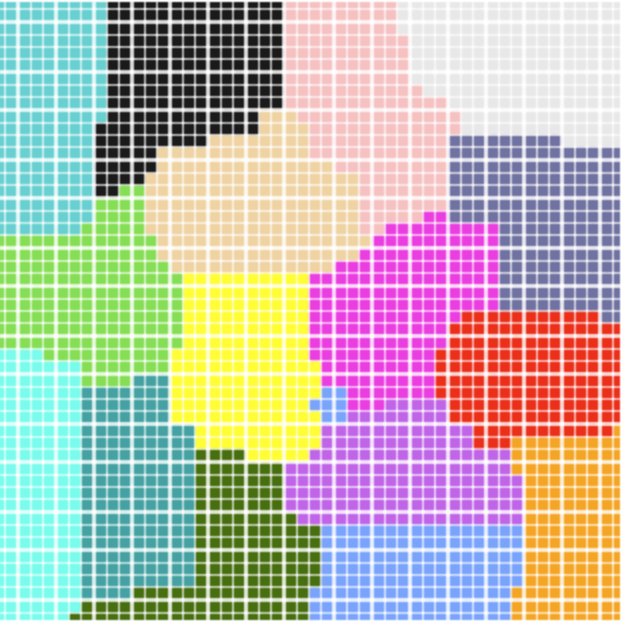
\includegraphics[width=0.6\textwidth]{images/noises/1}}
    \caption[short]{}
\end{subfigure}
\begin{subfigure}{.5\textwidth}
    \centering
    \fbox{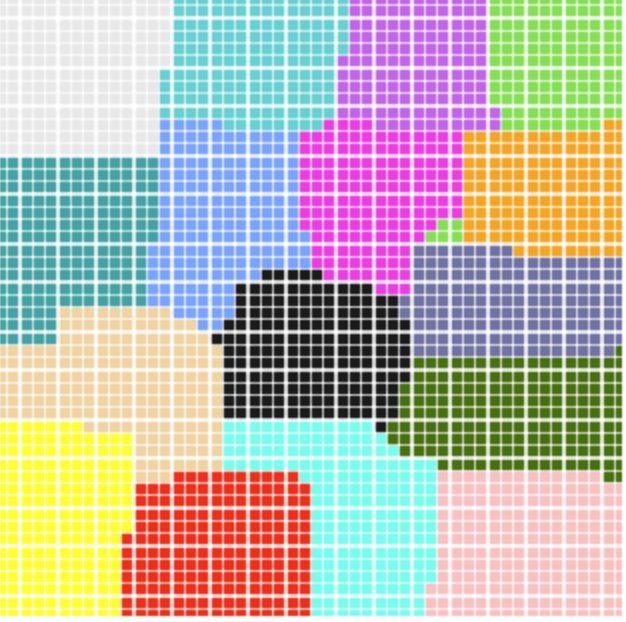
\includegraphics[width=0.6\textwidth]{images/noises/2}}
    \caption[short]{}
\end{subfigure}%
\caption{Na rysunku (a) widać, że niebieski obszar jest w dwóch miejscach - na dole oraz w postaci bardzo małego obszaru na środku.
Ten sam efekt występuje dla obszaru zielonego na obrazku (b).}
\label{im:noises}
\end{figure}

Problem spowodowany jest etapem optymalizacji podziału.
Dzieje się tak, ponieważ obszary handlują ze sobą granicznymi wierzchołkami w celu wyrównania granic.
Przykład podziału, na którym taki problem może się pojawić jest rysunek \ref{im:noises_2}.
W lewym rogu widać obszar zaznaczony czerwonym kółkiem, znajdujący się pomiędzy dwoma zielonymi obszarami.
Wąska, dolna odnoga tego obszaru jest potencjalnym miejscem, gdzie może nastąpić
odcięcie i przez to przedzielenie tego obszaru na dwie części.

\begin{figure}[h]
\centering
\fbox{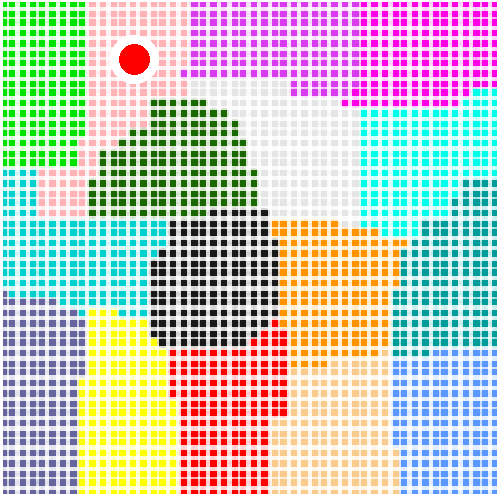
\includegraphics[width=0.3\textwidth]{images/noises/3}}
\caption{Na rysunku widać obraz siatki podatnej na pojawienie się obszarów rozproszonych. Czerwoną kropką zaznaczony jest obszar podatny
na podzielenie na dwie części.}
\label{im:noises_2}
\end{figure}

Algorytm optymalizacji granic jest szczególnie narażony na tego typu zachowania w swoich początkowych fazach,
kiedy graf jest zredukowany i pod pojedynczymi wierzchołkami przenoszone są tak naprawdę całe ich zbiory.
Wtedy często wystarczy przenieść jeden wierzchołek, aby przedzielić inny obszar na dwie części.
Dlatego też algorytm optymalizacji podziału aktywowany jest dopiero na grafie przywróconym w $85-90\%$ do
pierwotnego rozmiaru - wtedy szansa na powstanie obszarów rozproszonych znacznie spada.
Kolejnym czynnikiem ryzyka są obszary niepodzielne.
Reprezentują je wierzchołki, które zostają zastąpione początkowym zbiorem wierzchołków
dopiero po zakończeniu optymalizacji.
Przeniesienie takiego obszaru do innej partycji w fazie optymalizacji, tak samo jak w poprzednim przypadku, może skutkować
powstaniem obszarów rozproszonych.
Bardzo często również obszary rozproszone pojawiają się w początkowych wywołaniach optymalizacji granic, ale są niwelowane przez
kolejne wywołania algorytmu optymalizacji.
Ważnym faktem jest, że algorytm LAM ze względu na swoją charakterystykę dąży do budowania obszarów równych pod względem
pola oraz ''zbitych'', więc taka sytuacja nie zdarza się często.
Ponadto, jak wynika z moich obserwacji, pojawiające się obszary rozproszone są zawsze bardzo małe w
porównaniu do pozostałych obszarów.

Rozwiązanie dla tego problemu, które prezentuję w niniejszej pracy polega na pojedynczym przeiterowaniu po grafie
w celu znalezienia takich obszarów, następnie na przyporządkowaniu wszystkich obszarów rozproszonych do jednego
z przylegających do nich obszarów.
Algorytm usuwania obszarów rozproszonych jest wywoływany raz na grafie przywróconym do początkowych rozmiarów,
po wszystkich wywołaniach
algorytmu optymalizacji granic i wielkości pól.

Zdecydowałem się na tego typu, proste rozwiązanie z racji na rzadkość występowania tego problemu oraz tego, że zwykle
powstałe obszary rozproszone są bardzo małe.
Według mnie takie rozwiązanie jest dużo tańsze obliczeniowo i rozsądniejsze przy skali tego
zjawiska niż wykluczenie wystąpienia tego typu sytuacji dodatkowymi modyfikacjami algorytmu.